\documentclass[tikz,convert={density=800,outext=.png},border=5pt]{standalone}
%\documentclass[preview]{standalone}

\usepackage[utf8]{inputenc} % utf8 encoding

\usepackage{tikz}
\usetikzlibrary{positioning}

\begin{document}

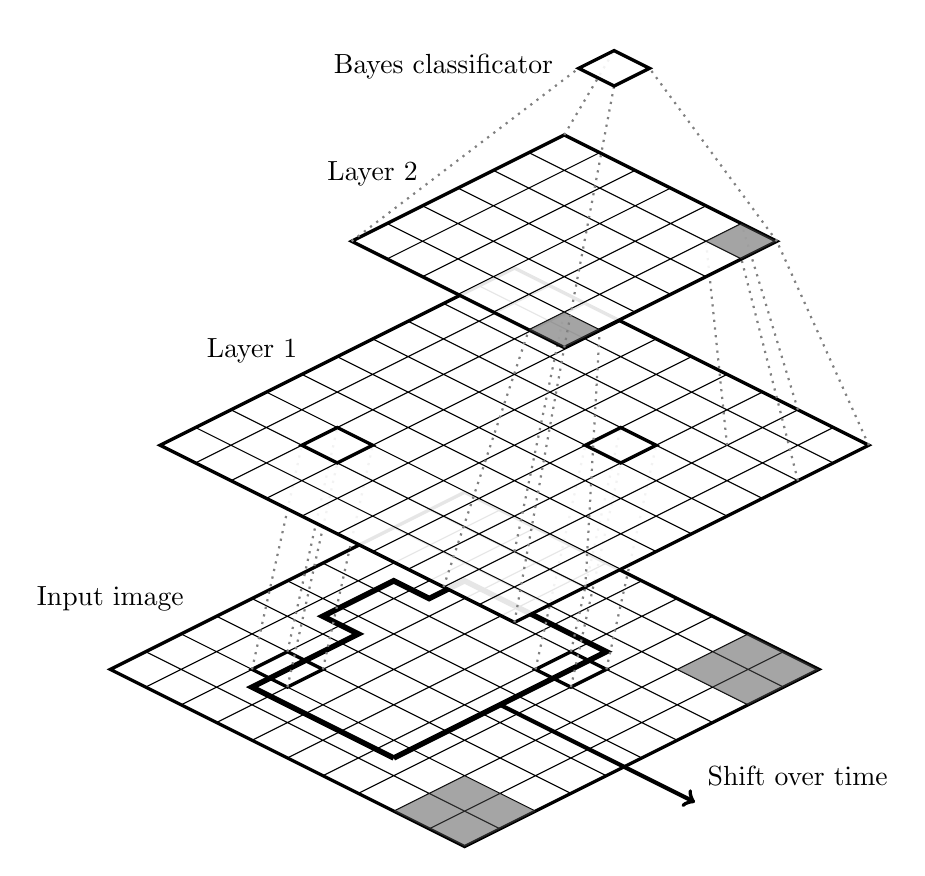
\begin{tikzpicture}[scale=.9,every node/.style={minimum size=1cm},on grid]          
    \begin{scope}[  % Lower layer
	    every node/.append style={
	    	yslant=0.5,xslant=-1},yslant=0.5,xslant=-1
	    ]
	    
	    \fill[white,fill opacity=.9] (0,0) rectangle (5,5);
	    \draw[step=5mm, black] (-1,-1) grid (4,4);
	    \draw[black,very thick] (-1,-1) rectangle (4,4);
	    \fill[black!70,opacity=0.5] (-1,-1) rectangle (0,0);
	    \fill[black!70,opacity=0.5] (4,-1) rectangle (3,0);
	    
	    \path[draw, line width=2pt, black] (-0.25,0.75) -- (2.75,0.75) -- (2.75,2.75) -- (2.25,2.75) -- (2.25,3.25) -- (1.25,3.25) -- (1.25,2.75) -- (-0.25,2.75) -- (-0.25,0.75);
	    \draw[black,very thick] (0.5,2.5) rectangle (0,3);
	    \draw[black,very thick] (2,1) rectangle (2.5,0.5);
	    
	    \coordinate (A) at (0,2.5); \coordinate (B) at (0.5,2.5); \coordinate (C) at (0,3); \coordinate (D) at (0.5,3);
	    \coordinate (E) at (2,1); \coordinate (F) at (2,0.5); \coordinate (G) at (2.5,1); \coordinate (H) at (2.5,0.5);
	    \draw[->,line width=1.5pt] (1.25, 0.75) -- (1.25,-2);
    \end{scope}
    
    \begin{scope}[  % Middle layer
        yshift=90,xshift=20,every node/.append style={
	        yslant=0.5,xslant=-1},yslant=0.5,xslant=-1
        ]
        \draw[gray,thick, dotted] (A) -- (0,2.5) (B) -- (0.5,2.5) (C) -- (0,3) (D) -- (0.5,3);
        \draw[gray,thick, dotted] (E) -- (2,1) (F) -- (2,0.5) (G) -- (2.5,1) (H) -- (2.5,0.5);
        \fill[white,fill opacity=.9] (-1,-1) rectangle (4,4);
        \draw[step=5mm, black] (-1,-1) grid (4,4);
        \draw[black,very thick] (-1,-1) rectangle (4,4);
        
		\draw[black,very thick] (2,1) rectangle (2.5,0.5);
        \draw[black,very thick] (0.5,2.5) rectangle (0,3);
        
        \coordinate (A) at (-1,-1); \coordinate (B) at (-1,0); \coordinate (C) at (0,-1); \coordinate (D) at (0,0);
        \coordinate (E) at (4,-1); \coordinate (F) at (4,0); \coordinate (G) at (3,-1); \coordinate (H) at (3,0);
    \end{scope}

    \begin{scope}[  % Upper layer
        yshift=115,xshift=40,every node/.append style={
            yslant=0.5,xslant=-1},yslant=0.5,xslant=-1
          ]
        \draw[gray,thick, dotted] (A) -- (2,2) (B) -- (2,2.5) (C) -- (2.5,2) (D) -- (2.5,2.5);
        \draw[gray,thick, dotted] (E) -- (5,2) (F) -- (5,2.5) (G) -- (4.5,2) (H) -- (4.5,2.5);
        \fill[white,fill opacity=0.9] (2,2) rectangle (5,5);
        \draw[step=5mm, black] (2,2) grid (5,5);
        \draw[black,very thick] (2,2) rectangle (5,5);

        \fill[black!70,opacity=0.5] (2,2) rectangle (2.5,2.5);
        \fill[black!70,opacity=0.5] (5,2) rectangle (4.5,2.5);
        
        \coordinate (A) at (2,2); \coordinate (B) at (2,5); \coordinate (C) at (5,2); \coordinate (D) at (5,5);
    \end{scope}
    
    \begin{scope}[  % Bayes layer
	    yshift=220,xshift=60,every node/.append style={
	    	yslant=0.5,xslant=-1},yslant=0.5,xslant=-1
		]
	    
	    \draw[gray,thick, dotted] (A) -- (2,2) (B) -- (2,2.5) (C) -- (2.5,2) (D) -- (2.5,2.5);
	    \fill[white,fill opacity=0.9] (2,2) rectangle (2.5,2.5);
	    \draw[black,very thick] (2,2) rectangle (2.5,2.5);
	    
    \end{scope}
    
    \node at (-5,2.5) {Input image};
    \node at (-3,6) {Layer 1};
    \node at (-1.3,8.5) {Layer 2};
    \node at (-0.3,10) {Bayes classificator};
    \node at (4.7,0) {Shift over time};
\end{tikzpicture}

\end{document}